\documentclass{scrartcl}
\usepackage[utf8]{inputenc}
\usepackage[english]{babel}
\usepackage{caption}
\usepackage{subcaption}
\usepackage{listings}
\usepackage{pdfpages}
\usepackage{amsmath,amssymb}
\usepackage{siunitx}
\usepackage{hyperref}
\usepackage{mhchem}
\usepackage[section]{placeins}
\usepackage[activate, protrusion=true, expansion=true]{microtype}
\usepackage[left=2.5cm, right=2.5cm, bottom=2.5cm, top=2.5cm]{geometry}
\usepackage{libertine}
\usepackage{longtable}

\newcommand{\qed}{\hfill $\blacksquare$}

\lstset{frame=single,keepspaces=true,captionpos=b}

\title{Digital 3D Geometry Processing}
\subtitle{Exercise 4}
\author{\textsc{Jannik Reichert} \and \textsc{Arne Sachtler} \and \textsc{Niklas Schmitz}}
\date{\today}

\begin{document}
\maketitle

\section{Theory Exercise}

\subsection{Curvature of Curves}

\begin{itemize}
	\item \textbf{1-d}: The function $k_1(s) = \frac{s^2 -1}{s^2+1}$ converges to $1$ for $\lim\limits_{s \rightarrow \infty} k_1(s)$ and $\lim\limits_{s \rightarrow -\infty} k_1(s)$. Figure~d shows a shape, where the curve converges to two different circles for large and largely negative $s$. The circle has constant curvature, that's why figure d matches the curvature function $k_1$.
	\item \textbf{2-a}: Figure a shows point-symmetry, therefore the curvature function must odd. The curvature is strictly positive when moving from the center right and strictly negative when moving left. Therefore, the curvature function $k_2$ matches.
	\item \textbf{3-c}: Figure c is also point-symmetric and $k_3$ is the remaining odd function.
	\item \textbf{4-b}: The periodicity of the sine can not hide.
\end{itemize}

\subsection{Surfaces Area}
% King Archimedes wants to renovate his palace. The most striking structure is a spherical
% half-dome of 20m in diameter that covers the great hall. The king wants to cover this
% dome in a layer of pure gold. He has decided to split the work into two parts, each one
% covering a vertical slice of the dome of the same height (see Figure 2). For each part he
% hires different people and gives them 700kg of gold. The task is to cover the surface of
% one vertical slice with a layer of gold of 0.1mm thickness. The amount of gold that is left
% over is the salary for doing the job. Which slice should you pick if you want to make the
% most profit? Explain your answer in TheoryExercise.pdf.
% How does your answer change when you have n slices instead of just two?

Preferable is the part, on which we have to use less gold to cover it.
We therefore calculate the surfaces of parts A and B.
As we at first only care about which area is smaller, we can calculate it on the 
unit (half-)sphere.
We parametrize similar to the mapping in lecture 4
\begin{equation}
	\mathbf{x}(u,v) = 
	\begin{pmatrix}
		cos\,u\,sin\,v\\
		sin\,u\,sin\,v\\
		cos\,v
	\end{pmatrix}
	,\quad
	\left(u,v\right)\in \left[0,2\pi\right)\times \left[0,\frac{\pi}{2}\right) \, .
\end{equation}
Note that we changed the range of the $v$ parameter as the desired shape is a hemi-sphere.
A handy tool for areas on surfaces is the first fundamental form, which turns out to be
\begin{equation}
	\mathbf{I} =
	\begin{pmatrix}
		E & F\\
		F & G
	\end{pmatrix}
	=
	\begin{pmatrix}
		{\mathbf{x}_{,u}}^\top{\mathbf{x}_{,u}} & {\mathbf{x}_{,u}}^\top{\mathbf{x}_{,v}}\\
		{\mathbf{x}_{,u}}^\top{\mathbf{x}_{,v}} & {\mathbf{x}_{,v}}^\top{\mathbf{x}_{,v}}
	\end{pmatrix}
	=
	\begin{pmatrix}
		sin^2\,v & 0\\
		0 & 1
	\end{pmatrix}\, .
\end{equation}
We first observe that the choice of the part is independent of the radius. The area for part B on a unit hemi-sphere can be calculated using
\begin{eqnarray}
	\int_0^{\frac{\pi}{4}}\int_0^{2\pi} \sqrt{EG-F^2} \, du \, dv
	\underset{v \ge 0}{=}\int_0^{\frac{\pi}{4}}\int_0^{2\pi} sin(v) \, du \, dv
	&=&\int_0^{\frac{\pi}{4}}[u\,sin\,v]_0^{2\pi} \, dv \\\nonumber
	=2\pi\int_0^{\frac{\pi}{4}}sin\,v\,dv
	&=&2\pi(-\sqrt{2}+1)\\\nonumber
	&=&(2-\sqrt{2})\pi\, .
\end{eqnarray}
As a hemi-sphere has the total area $2\pi$, part A has the area
$\sqrt{2}\pi=2\pi-((2-\sqrt{2})\pi)$, which makes it larger than part B.
Instead of using this approach, it is also possible to compute the area by integrating over $v \in \left[\frac{\pi}{4}, \frac{\pi}{2}\right]$.
Part B is preferable as the surface area is smaller.

\subsubsection*{How about N slices?}
Slicing the hemi-sphere into $N$ slices in height leads to equal-length stripes in the parameter space.
Let $a = \frac{i-1}{2N}\pi$ and $b = \frac{i}{2N}\pi$ for $i \in [1, \ldots, N]$. Then, the area of the $i$-th slice $A_i$ can computed by
\begin{eqnarray}
	A_i &=& \int\limits_a^b \int\limits_0^{2\pi} \sin(v) du\, dv\\
	&=& \int\limits_a^b \sin(v) \left(\int_0^{2\pi} du\right)dv\\\nonumber
	&=& \int\limits_a^b 2\pi \sin(v) dv\nonumber
\end{eqnarray}
In the limit case for $N \rightarrow \infty$ we obtain a density function
\begin{equation}
	f(v) = 2\pi \sin(v)\, ,
\end{equation}
which yields the \emph{area per height} dependent on the (normalized) height $v$. This is a density as $\int_{v_1}^{v_2} f(v)dv$ computes the surface of the hemi-sphere between $v_1$ and $v_2$. Plotting this density function leads to the image shown in Figure~\ref{fig:area_density}.
\begin{figure}[h]
	\centering
	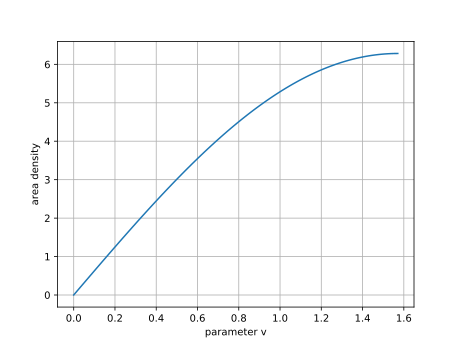
\includegraphics[height=7cm]{figures/density.pdf}
	\caption{Density function of area per parameter $v$.}
	\label{fig:area_density}
\end{figure}

\noindent
Slicing the hemi-sphere into $N$ slices leads to equidistant slicing of the $v$ axis in the parameter space.
The surface area of one of the slices is then the integral of the area-density $f(v)$ over the slice bound in $v$. Therefore, one should always pick the bottommost slice as its area is smallest.
\end{document}
